\documentclass{article}\usepackage[]{graphicx}\usepackage[]{color}
%% maxwidth is the original width if it is less than linewidth
%% otherwise use linewidth (to make sure the graphics do not exceed the margin)
\makeatletter
\def\maxwidth{ %
  \ifdim\Gin@nat@width>\linewidth
    \linewidth
  \else
    \Gin@nat@width
  \fi
}
\makeatother

\definecolor{fgcolor}{rgb}{0.345, 0.345, 0.345}
\newcommand{\hlnum}[1]{\textcolor[rgb]{0.686,0.059,0.569}{#1}}%
\newcommand{\hlstr}[1]{\textcolor[rgb]{0.192,0.494,0.8}{#1}}%
\newcommand{\hlcom}[1]{\textcolor[rgb]{0.678,0.584,0.686}{\textit{#1}}}%
\newcommand{\hlopt}[1]{\textcolor[rgb]{0,0,0}{#1}}%
\newcommand{\hlstd}[1]{\textcolor[rgb]{0.345,0.345,0.345}{#1}}%
\newcommand{\hlkwa}[1]{\textcolor[rgb]{0.161,0.373,0.58}{\textbf{#1}}}%
\newcommand{\hlkwb}[1]{\textcolor[rgb]{0.69,0.353,0.396}{#1}}%
\newcommand{\hlkwc}[1]{\textcolor[rgb]{0.333,0.667,0.333}{#1}}%
\newcommand{\hlkwd}[1]{\textcolor[rgb]{0.737,0.353,0.396}{\textbf{#1}}}%
\let\hlipl\hlkwb

\usepackage{framed}
\makeatletter
\newenvironment{kframe}{%
 \def\at@end@of@kframe{}%
 \ifinner\ifhmode%
  \def\at@end@of@kframe{\end{minipage}}%
  \begin{minipage}{\columnwidth}%
 \fi\fi%
 \def\FrameCommand##1{\hskip\@totalleftmargin \hskip-\fboxsep
 \colorbox{shadecolor}{##1}\hskip-\fboxsep
     % There is no \\@totalrightmargin, so:
     \hskip-\linewidth \hskip-\@totalleftmargin \hskip\columnwidth}%
 \MakeFramed {\advance\hsize-\width
   \@totalleftmargin\z@ \linewidth\hsize
   \@setminipage}}%
 {\par\unskip\endMakeFramed%
 \at@end@of@kframe}
\makeatother

\definecolor{shadecolor}{rgb}{.97, .97, .97}
\definecolor{messagecolor}{rgb}{0, 0, 0}
\definecolor{warningcolor}{rgb}{1, 0, 1}
\definecolor{errorcolor}{rgb}{1, 0, 0}
\newenvironment{knitrout}{}{} % an empty environment to be redefined in TeX

\usepackage{alltt}
\usepackage{statrep}
\usepackage{hyperref}
\usepackage{parskip,xspace}
\def\SRrootdir{/folders/myshortcuts/report-example/code}
\def\SRmacropath{/folders/myshortcuts/sas-macros/statrep/statrep_macros.sas}
\title{Streamline Your Workflow: Integrating SAS, LaTeX, and R into a Single Reproducible Document \emph{A 538 Star Wars Example}}
\author{Lucy D'Agostino McGowan}
\date{\today}
\IfFileExists{upquote.sty}{\usepackage{upquote}}{}
\begin{document}
\maketitle
\section{Introduction}

I obtained data from a 538 Star Wars Survey (found here: \url{https://github.com/fivethirtyeight/data/tree/master/star-wars-survey}) and will read it into SAS in order to analyze whether age, gender, or education level are associated with incorrectly believing that Greedo shot first.

\begin{Sascode}
libname data "/folders/myshortcuts/report-example/data";

filename reffile 
  '/folders/myshortcuts/report-example/data/star-wars-survey-538.csv';

proc import datafile=reffile
	dbms=csv
	replace
	out=data.starwars;
	getnames=yes;
run;
\end{Sascode}

\begin{Sascode}
data data;
 set data.starwars;
  if Jar_Jar_Binks in (" ", "Unfamiliar (N/A)")
    then wrong_jar_jar = " ";
  else if Jar_Jar_Binks in ("Very favorably","Somewhat favorably") 
    then wrong_jar_jar = 1;
    else wrong_jar_jar = 0;
  if shot_first = "Han" 
    then wrong_han = 0;
  if shot_first = "Greedo" 
    then wrong_han = 1;
  if education in ("Bachelor degree", "Graduate degree") 
    then college = "College degree";
  if education in ("Some college or Associate degree", 
    "High school degree", "Less than high school degree") 
    then college = "No college degree";
run;

\end{Sascode}

\begin{Sascode}[store=freq]
ods graphics on;

proc freq data = data;
table wrong_han wrong_jar_jar;
run;

ods graphics off;
\end{Sascode}

\Listing[caption = {Wrong about who shot first}, 
    store = freq,
    objects = Freq.Table1.OneWayFreqs]{freqtabhan}

\Listing[caption={Wrong aboud Jar Jar Binks}, 
    store=freq,
    objects = Freq.Table2.OneWayFreqs]{freqtabjar}

\begin{Sascode}[store = logistic]
ods graphics on;

proc logistic data = data plots = oddsratio;
 class age (ref = FIRST) gender college Star_Trek_fan;
 model wrong_han(event = "1") = age gender college Star_Trek_fan;
run;

ods graphics off;
\end{Sascode}

\begin{Sascode}[store = logisticj]
ods graphics on;

proc logistic data = data plots = oddsratio;
 class age (ref = FIRST) gender college Star_Trek_fan;
 model wrong_jar_jar(event = "1") = age gender college Star_Trek_fan;
run;

ods graphics off;
\end{Sascode}

\Listing[caption = {Wrong about who shot first Odds Ratio},
store = logistic,
objects = OddsRatios]{logisticOR}

\Graphic[store=logistic,
   objects=ORPlot,
   caption={Wrong about Jar Jar Binks}]{ORplot}

\Listing[caption = {Wrong about who shot first Odds Ratio},
store = logisticj,
objects = OddsRatios]{logisticORj}

\Graphic[store=logisticj,
   objects=ORPlot,
   caption={Wrong about Jar Jar Binks}]{ORplotj}


\begin{Sascode}
proc export data=data.starwars
   outfile =
     '/folders/myshortcuts/report-example/data/starwars_sasedit.csv'
   replace
   dbms = dlm;
   delimiter = ',';
run;
\end{Sascode}

\section{Test}

\begin{knitrout}
\definecolor{shadecolor}{rgb}{0.969, 0.969, 0.969}\color{fgcolor}\begin{kframe}
\begin{alltt}
\hlstd{filename} \hlkwb{=} \hlstr{"../data/starwars_sasedit.csv"}
\hlkwa{if} \hlstd{(}\hlkwd{file.exists}\hlstd{(filename))\{}
  \hlcom{#load libraries}
  \hlkwd{library}\hlstd{(}\hlstr{'dplyr'}\hlstd{)}
  \hlkwd{library}\hlstd{(}\hlstr{'rphylopic'}\hlstd{)}
  \hlkwd{library}\hlstd{(}\hlstr{'png'}\hlstd{)}
  \hlkwd{library}\hlstd{(}\hlstr{'ggplot2'}\hlstd{)}

  \hlcom{#read in data}
  \hlstd{starwars} \hlkwb{<-} \hlkwd{read.csv}\hlstd{(filename)}

  \hlcom{#load some cute pics}
  \hlstd{chewie} \hlkwb{<-} \hlkwd{readPNG}\hlstd{(}\hlstr{"../data/img/chewie.png"}\hlstd{)}
  \hlstd{stormtrooper} \hlkwb{<-} \hlkwd{readPNG}\hlstd{(}\hlstr{"../data/img/storm_trooper.png"}\hlstd{)}


  \hlstd{starwars} \hlopt
    \hlkwd{filter}\hlstd{(shot_first} \hlopt \hlkwd{c}\hlstd{(}\hlstr{"Han"}\hlstd{,}\hlstr{"Greedo"}\hlstd{))} \hlopt
    \hlkwd{select}\hlstd{(shot_first,The_Phantom_Menace,}
           \hlstd{Attack_of_the_Clones,Revenge_of_the_Sith,}
           \hlstd{A_New_Hope,The_Empire_Strikes_Back,}
           \hlstd{Return_of_the_Jedi)} \hlopt
    \hlkwd{group_by}\hlstd{(shot_first)} \hlopt
    \hlkwd{summarise_each}\hlstd{(}\hlkwd{funs}\hlstd{(}\hlkwd{mean}\hlstd{(.,} \hlkwc{na.rm} \hlstd{=} \hlnum{TRUE}\hlstd{)))}  \hlopt
    \hlstd{tidyr}\hlopt{::}\hlkwd{gather}\hlstd{(}\hlstr{"film"}\hlstd{,}\hlstr{"rank"}\hlstd{,}\hlnum{2}\hlopt{:}\hlnum{7}\hlstd{)} \hlopt
    \hlkwd{mutate}\hlstd{(}\hlkwc{film} \hlstd{=} \hlkwd{gsub}\hlstd{(}\hlstr{"_"}\hlstd{,} \hlstr{" "}\hlstd{, film))} \hlopt
    \hlkwd{data.frame}\hlstd{()} \hlkwb{->} \hlstd{plot_data}
 \hlstd{plot_data}\hlopt{$}\hlstd{film} \hlkwb{<-} \hlkwd{reorder}\hlstd{(plot_data}\hlopt{$}\hlstd{film,} \hlkwd{rep}\hlstd{(}\hlnum{1}\hlopt{:}\hlnum{6}\hlstd{,} \hlkwc{each} \hlstd{=} \hlnum{2}\hlstd{))}
 \hlstd{p} \hlkwb{<-}  \hlkwd{ggplot}\hlstd{(plot_data,}\hlkwd{aes}\hlstd{(film, rank,} \hlkwc{group} \hlstd{= shot_first))}  \hlopt{+}
   \hlkwd{geom_line}\hlstd{(}\hlkwd{aes}\hlstd{(}\hlkwc{color} \hlstd{= shot_first))} \hlopt{+}
   \hlkwd{scale_colour_manual}\hlstd{(}\hlkwc{values} \hlstd{=} \hlkwd{c}\hlstd{(}\hlstr{"black"}\hlstd{,}\hlstr{"brown"}\hlstd{))} \hlopt{+}
   \hlkwd{ylim}\hlstd{(}\hlnum{0}\hlstd{,}\hlnum{6}\hlstd{)}
   \hlkwa{for} \hlstd{(i} \hlkwa{in} \hlnum{1}\hlopt{:}\hlnum{6}\hlstd{) \{}
   \hlstd{p} \hlkwb{<-} \hlstd{p} \hlopt{+} \hlkwd{add_phylopic}\hlstd{(chewie,} \hlnum{1}\hlstd{, i,}
                         \hlstd{plot_data[plot_data}\hlopt{$}\hlstd{shot_first}\hlopt{==}\hlstr{"Han"}\hlstd{,}
                                   \hlstr{"rank"}\hlstd{][i],}
                         \hlkwc{ysize} \hlstd{=} \hlnum{1}\hlstd{)}
   \hlstd{\}}
    \hlkwa{for} \hlstd{(i} \hlkwa{in} \hlnum{1}\hlopt{:}\hlnum{6}\hlstd{) \{}
   \hlstd{p} \hlkwb{<-} \hlstd{p} \hlopt{+} \hlkwd{add_phylopic}\hlstd{(stormtrooper,} \hlnum{1}\hlstd{, i,}
                         \hlstd{plot_data[plot_data}\hlopt{$}\hlstd{shot_first}\hlopt{==}\hlstr{"Greedo"}\hlstd{,}
                                   \hlstr{"rank"}\hlstd{][i],}
                         \hlkwc{ysize} \hlstd{=} \hlnum{1}\hlstd{)}
 \hlstd{\}}
 \hlstd{p} \hlopt{+}
   \hlkwd{ggtitle}\hlstd{(}\hlstr{"Star Wars Film Rankings by Who Shot First"}\hlstd{)} \hlopt{+}
   \hlkwd{theme}\hlstd{(}\hlkwc{axis.text.x} \hlstd{=} \hlkwd{element_text}\hlstd{(}\hlkwc{angle} \hlstd{=} \hlnum{60}\hlstd{,} \hlkwc{hjust} \hlstd{=} \hlnum{1}\hlstd{))}
\hlstd{\}}
\end{alltt}
\end{kframe}
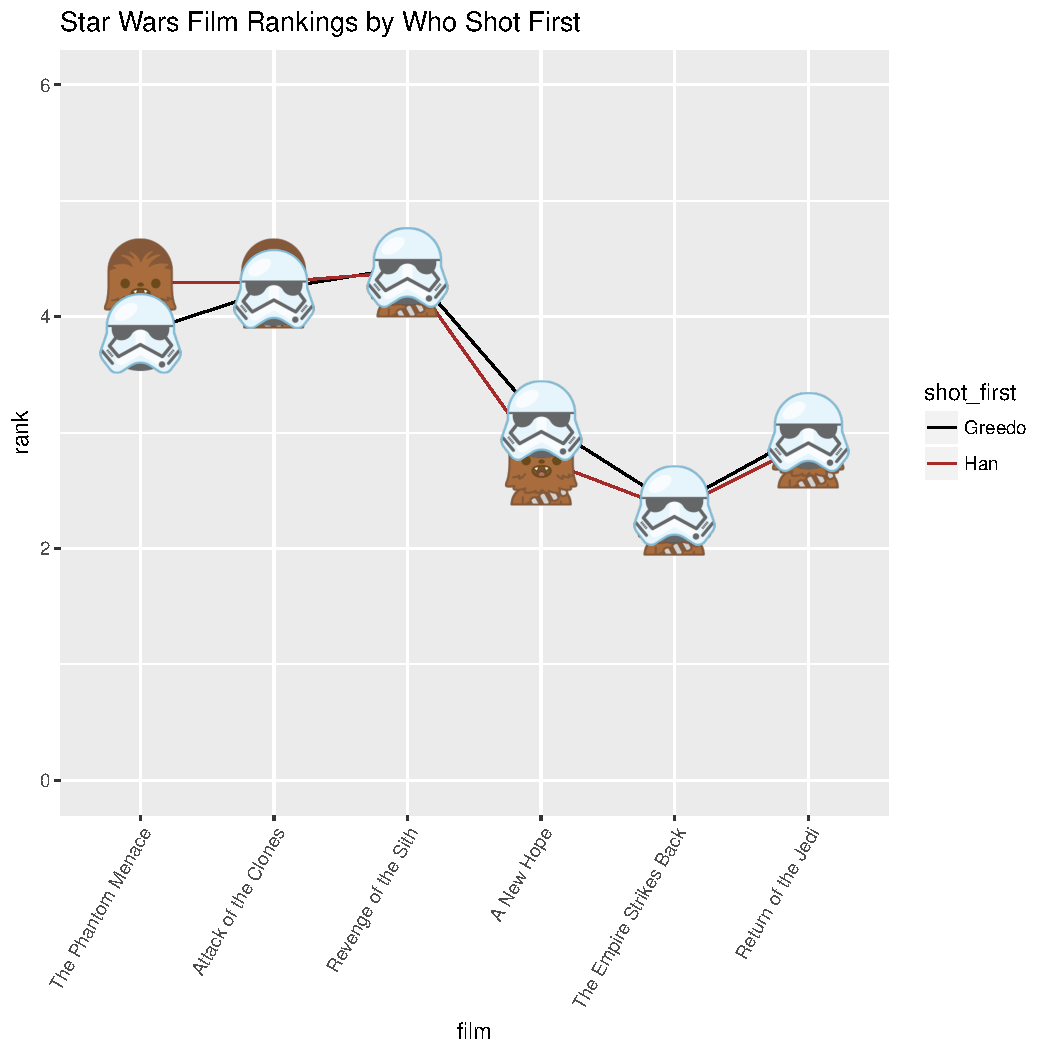
\includegraphics[width=\maxwidth]{figure/unnamed-chunk-1-1} 

\end{knitrout}

\end{document}
